\documentclass[12pt, twoside, openany]{book}
%\documentclass[12pt, oneside]{book}  % jednostranna tlac
\linespread{1.25} % hodnota 1.25 by mala zodpovedat 1.5 riadkovaniu
\pagestyle{plain}
% -------------------
% --- Packages
% -------------------
\usepackage[a4paper,top=2.5cm,bottom=2.5cm,left=3.5cm,right=2cm]{geometry}
\usepackage[utf8]{inputenc}
\usepackage[T1]{fontenc}
\usepackage{graphicx}
\usepackage{url}

% --- additional packages
\usepackage{epsfig}
\usepackage{epstopdf}
%\usepackage[chapter]{algorithm}
\usepackage{algorithmic}
%\usepackage{listings}
\usepackage{amsmath}
\usepackage{amssymb}
\usepackage{multirow}
\usepackage{booktabs}
\usepackage{color}
\usepackage{setspace}
\usepackage{tabularx}
\usepackage{textcomp}
\usepackage{caption}
\usepackage{natbib}
\usepackage{subcaption}
\usepackage[font=large]{subcaption}
\usepackage{emptypage}
\usepackage{float}
\usepackage[hidelinks,breaklinks]{hyperref}
\usepackage{minted}
\usepackage[thinlines]{easytable}
\usepackage{amsmath}

%\captionsetup[subfigure]{font=large}




%aby sa nevykreslovali obrazky
%\renewcommand{\includegraphics}[2][]{
	%   \fbox{#2}% print file name in a small box
	%}


% -------------------
% --- Definicia zakladnych pojmov
% -------------------
\def\mfrok{2026}
\def\mftitle{Automatic generation of enemies in a survival computer game}
\def\mfthesistype{Master thesis}
\def\mfauthor{Michal Baránek}
\def\mfsupervisor{Ing. Alexander Šimko, PhD.}
\def\mfplacedate{Bratislava, 2025}
\def\mfuniversity{COMENIUS UNIVERSITY IN BRATISLAVA}
\def\mffaculty{FACULTY OF MATHEMATICS PHYSICS AND INFORMATICS}
\def\mfbranch{Applied informatics}
\def\program{Applied informatics}
\def\mfdepartment{Department of Applied Informatics}

\begin{document}
	\frontmatter
	
	
	% -------------------
	% --- Obalka ------
	% -------------------
	\thispagestyle{empty}
	
	\noindent
	\begin{minipage}{\textwidth}
		\begin{center}
			\textbf{\mfuniversity \\
				\mffaculty}
		\end{center}
	\end{minipage}
	
	\vfill
	\begin{figure}[!hbt]
		\begin{center}
			
\includegraphics[width=0.4\textwidth]{images/FMFI_logo_BP.png}
			\label{img:logo}
		\end{center}
	\end{figure}
	\begin{center}
		\textbf{\MakeUppercase{\Large\mftitle}}\\
		\mfthesistype
	\end{center}
	\vfill
	\mfrok \hfill
	\mfauthor
	%\eject 
	\cleardoublepage
	% --- koniec obalky ----
	
	
	
	% -------------------
	% --- Titulný list
	% -------------------
	\thispagestyle{empty}
	\noindent
	\begin{minipage}{\textwidth}
		\begin{center}
			\textbf{\mfuniversity \\
				\mffaculty}
		\end{center}
	\end{minipage}
	
	\vfill
	\begin{figure}[!hbt]
		\begin{center}
			
\includegraphics[width=0.4\textwidth]{images/FMFI_logo_BP.png}
			\label{img:logo_dark}
		\end{center}
	\end{figure}
	
	\begin{center}
		\textbf{\MakeUppercase{\Large\mftitle}}\\
		\mfthesistype
	\end{center}
	\vfill
	
	
	\begin{tabular}{l l}
		Study program: & \program \\
		Branch of study: & \mfbranch \\
		Department: & \mfdepartment \\
		Supervisor: & \mfsupervisor \\
	\end{tabular}
	
	\vfill
	\noindent
	\mfplacedate \hfill
	\mfauthor
	%\eject 
	\cleardoublepage
	% --- Koniec titulnej strany
	
	
	
	% -------------------
	% --- Zadanie z AIS
	% -------------------
	% v tlačenej verzii s podpismi zainteresovaných osôb.
	% v elektronickej verzii sa zverejňuje zadanie bez podpisov
	% v pracach v naglictine anglicke aj slovenske zadanie
	
	\newpage 
	\thispagestyle{empty}
	\hspace{-2cm}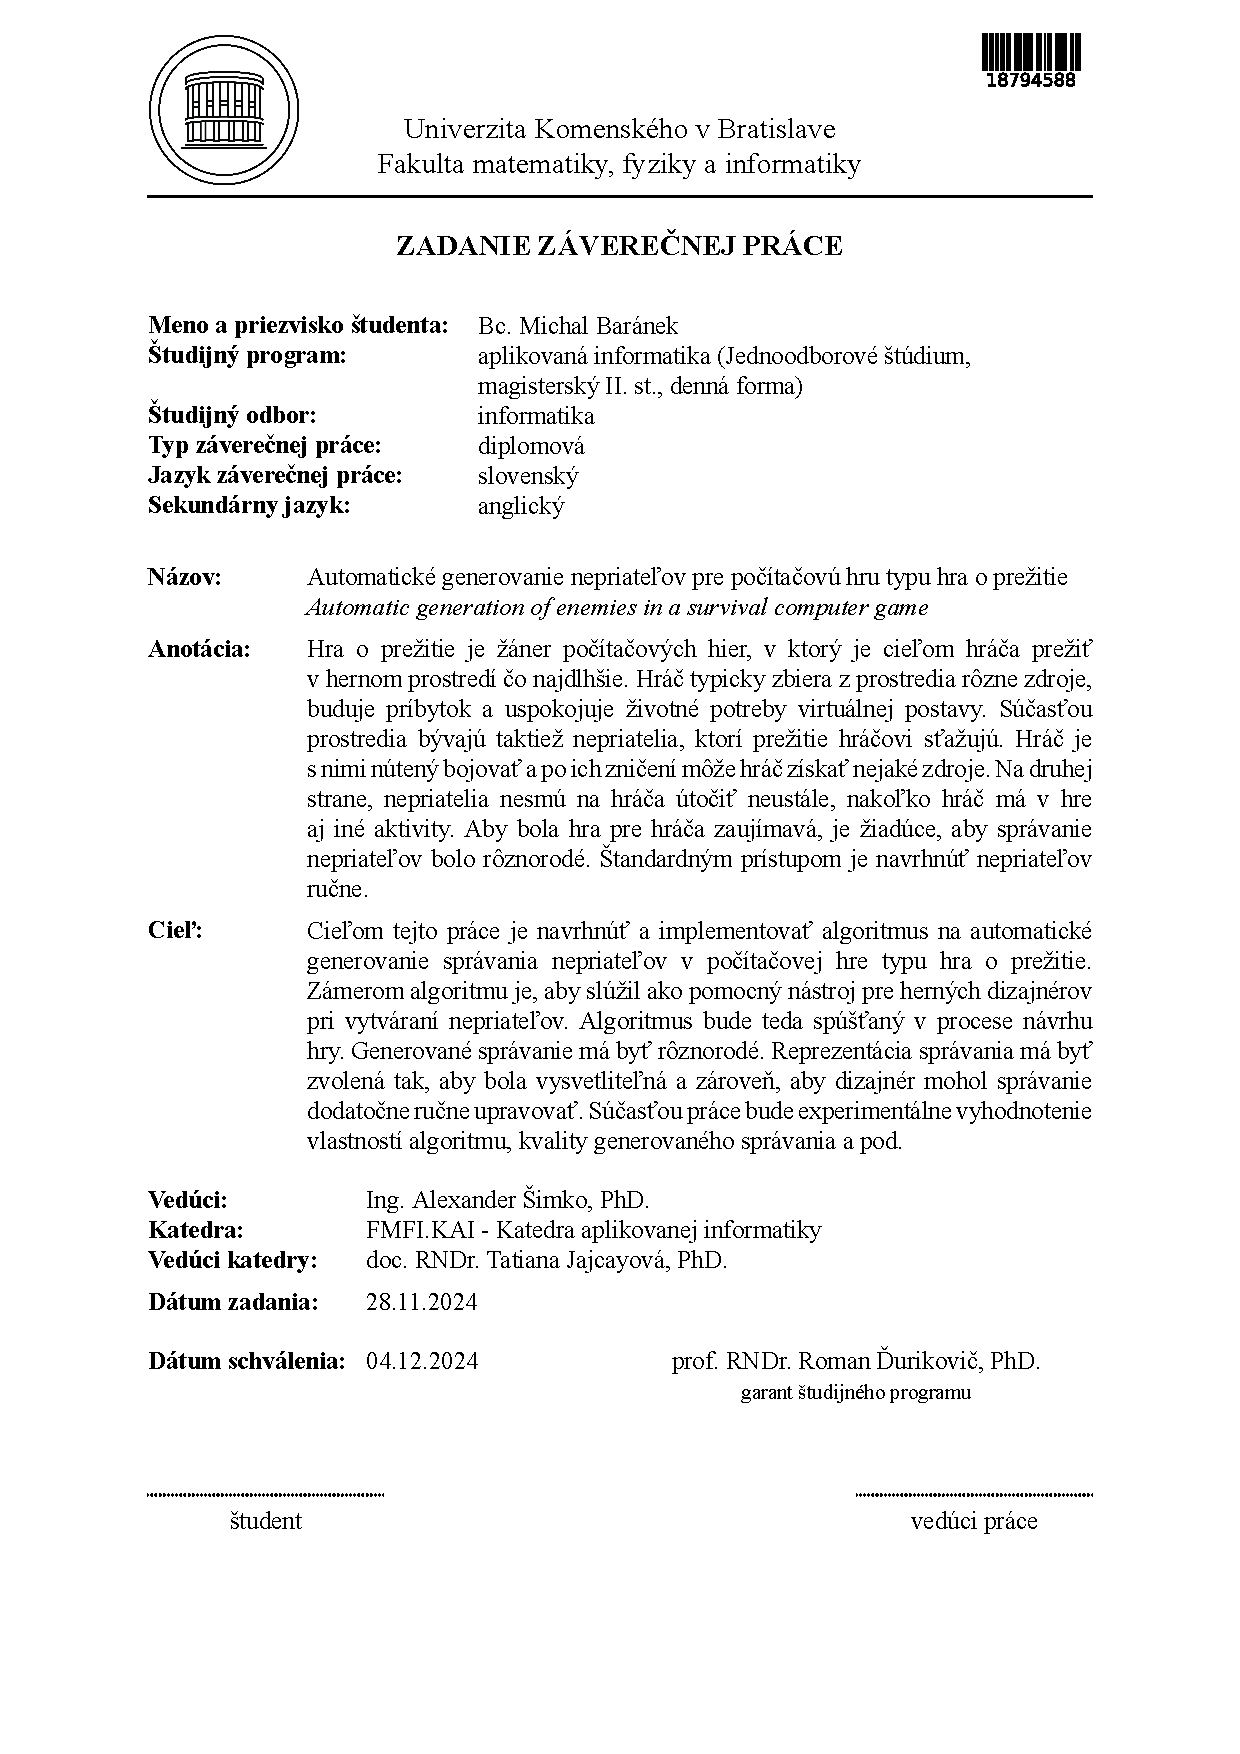
\includegraphics[page=1,width=1.1\textwidth]{zadanie.pdf}
	
	\newpage 
	\thispagestyle{empty}
	
	% --- Koniec zadania
	
	
	% -------------------
	% --- Prehlásenie
	% -------------------
	
	{~}\vspace{12cm}
	
	\noindent
	\begin{minipage}{0.25\textwidth}~\end{minipage}
	\thispagestyle{empty}
	\begin{minipage}{0.75\textwidth}
		I hereby declare that I have written this thesis by myself, only with help of referenced literature, under the careful supervision of my thesis advisor.
		\newline \newline
	\end{minipage}
	\vfill
	~ \hfill {\hbox to 6cm{\dotfill}} \\
	\mfplacedate \hfill \mfauthor
	\vfill\eject \cleardoublepage
	% --- koniec prehlasenia
	
	
	
	
	% -------------------
	% --- Poďakovanie
	% -------------------
	\newpage
	\thispagestyle{empty}
	\chapter*{Acknowledgement}\label{chap:thank_you}
	
	
	\vfill\eject 
	% --- koniec podakovania
	
	
	
	% -------------------
	% --- Abstrakty
	% -------------------
	\newpage 
	\thispagestyle{empty}
	\chapter*{Abstract}\label{chap:abstract_en}
	
	\paragraph*{Keywords:}  
	
	
	\newpage 
	\thispagestyle{empty}
	\chapter*{Abstrakt}\label{chap:abstract_sk}
	
	\paragraph*{Kľúčové slová:}
	
	
	% --- koniec abstraktov
	
	
	% -------------------
	% --- Obsah
	% -------------------
	\newpage 
	\tableofcontents
	
	% ---  Koniec Obsahu
	
	
	% -------------------
	% --- Zoznamy tabuliek, obrázkov - nepovinne
	% -------------------
	\newpage 
	\listoffigures
	\listoftables
	% ---  Koniec Zoznamov
	
	% \input{terminology}
	
	
	\mainmatter
	
	%main content 
	\chapter{Introduction}
	\section{Motivation}
	\section{Problem Statement}
	\section{Goals of the Thesis}
	\section{Structure of the Thesis}
	
	\chapter{Background and Related Work}
	\section{Survival Games: Genre Overview}
	\section{Enemy Design in Games}
	\section{Procedural Content Generation (PCG)}
	\section{Behavior Modeling Techniques}
	\subsection{Rule-based Systems}
	\subsection{Behavior Trees and Finite State Machines}
	\subsection{Evolutionary Algorithms in Game Design}
	\section{Summary}
	
	\chapter{Design of the Enemy Behavior Generator}
	\section{Design Objectives and Requirements}
	\section{Behavior Representation}
	\subsection{Explainability and Manual Adjustability}
	\section{Behavior Diversity and Gameplay Balance}
	\section{Overview of the Generation Pipeline}
	\section{Designer Interaction and Control Parameters}
	\section{Design Considerations}
	
	\chapter{Evolutionary Algorithm Design}
	\section{Overview of Evolutionary Algorithms}
	\subsection{Genetic Algorithms}
	\subsection{Representation of Individuals (Behaviors)}
	\subsection{Fitness Function Design}
	\section{Mutation and Crossover Strategies}
	\section{Selection and Population Management}
	\section{Termination Criteria}
	\section{Adaptation to Game Design Constraints}
	
	\chapter{Implementation}
	\section{Technology Stack}
	\section{System Architecture}
	\section{Key Modules}
	\subsection{Behavior Encoding and Decoding}
	\subsection{Evolution Engine}
	\subsection{Integration with Game Prototype}
	\section{Example Generated Behaviors}
	
	\chapter{Experimental Evaluation}
	\section{Experiment Setup}
	\subsection{Test Scenarios and Inputs}
	\subsection{Evaluation Metrics}
	\section{Results}
	\subsection{Behavior Diversity and Novelty}
	\subsection{Behavior Quality and Playability}
	\subsection{Performance Analysis}
	\section{Discussion}
	
	\chapter{Conclusion}
	\section{Summary of Contributions}
	\section{Limitations and Challenges}
	\section{Suggestions for Future Work}
	
	
	% -------------------
	% --- Bibliografia
	% -------------------
	
	\backmatter
	
	\nocite{*}
	\bibliographystyle{plain}
	\bibliography{references}
	
	%---koniec bibliografie
	
\end{document}